\documentclass[10pt,letterpaper]{article}
\usepackage[top=0.85in,left=1.5in,footskip=0.75in]{geometry}

% amsmath and amssymb packages, useful for mathematical formulas and symbols
\usepackage{amsmath,amssymb}

% Use adjustwidth environment to exceed column width (see example table in text)
\usepackage{changepage}

\usepackage{longtable}
\usepackage{caption}
\usepackage{subcaption}
\usepackage[label font=bf,labelformat=simple]{subfig}
\usepackage{floatrow}
\floatsetup[figure]{style=plain,subcapbesideposition=top}
\usepackage{parskip}
\usepackage{float}
\floatstyle{plaintop}
\restylefloat{table}
\usepackage{pdflscape}
\usepackage{afterpage}
\usepackage{minted}
% textcomp package and marvosym package for additional characters
\usepackage{textcomp,marvosym}

% cite package, to clean up citations in the main text. Do not remove.
%%\usepackage{cite}

% Use nameref to cite supporting information files (see Supporting Information section for more info)
\usepackage{nameref,hyperref}

% line numbers
\usepackage[right]{lineno}

% ligatures disabled
\usepackage[nopatch=eqnum]{microtype}
\DisableLigatures[f]{encoding = *, family = * }

% color can be used to apply background shading to table cells only
\usepackage[table]{xcolor}

% array package and thick rules for tables
\usepackage{array}

% create "+" rule type for thick vertical lines
\newcolumntype{+}{!{\vrule width 2pt}}

% create \thickcline for thick horizontal lines of variable length
\newlength\savedwidth
\newcommand\thickcline[1]{%
  \noalign{\global\savedwidth\arrayrulewidth\global\arrayrulewidth 2pt}%
  \cline{#1}%
  \noalign{\vskip\arrayrulewidth}%
  \noalign{\global\arrayrulewidth\savedwidth}%
}

% \thickhline command for thick horizontal lines that span the table
\newcommand\thickhline{\noalign{\global\savedwidth\arrayrulewidth\global\arrayrulewidth 2pt}%
\hline
\noalign{\global\arrayrulewidth\savedwidth}}


% Remove comment for double spacing
%\usepackage{setspace} 
%\doublespacing

% Text layout
\raggedright
\setlength{\parindent}{0.5cm}
\textwidth 5.25in 
\textheight 8.75in

% Bold the 'Figure #' in the caption and separate it from the title/caption with a period
% Captions will be left justified
\usepackage[aboveskip=1pt,labelfont=bf,labelsep=period,justification=raggedright,singlelinecheck=off]{caption}
\renewcommand{\figurename}{Fig}

% Use the PLoS provided BiBTeX style
\bibliographystyle{plos2015}

% Remove brackets from numbering in List of References
\makeatletter
\renewcommand{\@biblabel}[1]{\quad#1.}
\makeatother



% Header and Footer with logo
\usepackage{lastpage,fancyhdr,graphicx}
\usepackage{epstopdf}
%\pagestyle{myheadings}
\pagestyle{fancy}
\fancyhf{}
%\setlength{\headheight}{27.023pt}
%\lhead{\includegraphics[width=2.0in]{PLOS-submission.eps}}
\rfoot{\thepage/\pageref{LastPage}}
\renewcommand{\headrulewidth}{0pt}
\renewcommand{\footrule}{\hrule height 2pt \vspace{2mm}}
\fancyheadoffset[L]{2.25in}
\fancyfootoffset[L]{2.25in}
\lfoot{\today}

%% Include all macros below

\newcommand{\lorem}{{\bf LOREM}}
\newcommand{\ipsum}{{\bf IPSUM}}

%% END MACROS SECTION

%% Hy's package
%% For graphic/image
\usepackage{graphicx}
\usepackage{ragged2e}
\graphicspath{ {./figure/} }

%% For cite
\usepackage[style=apa, backend=biber]{biblatex}
\addbibresource{ref.bib}

% For caption to be smaller
\usepackage[font=small,labelfont=bf]{caption}

% For url
\usepackage{xurl}

% For line break
\usepackage{microtype}

% For supplement numbering
\newcommand{\beginsupplement}{%
        \setcounter{table}{0}
        \renewcommand{\thetable}{S\arabic{table}}%
        \setcounter{figure}{0}
        \renewcommand{\thefigure}{S\arabic{figure}}%
     }

\begin{document}
\vspace*{0.2in}

\begin{flushleft}
{\Large
\begin{center}
\textbf\newline{Expanding the DNA-probe toolbox for molecular profiling of tissues and their microbiomes}
\end{center}
}
\bigskip
\bigskip
Pham Xuan Huy Nguyen\textsuperscript{1,*}

\bigskip
\textsuperscript{1}Department of Biology, Lund University, Lund, Sweden
\bigskip
\newline
\newline
Supervisor: Nils Norlin
\bigskip
\newline
E-mail: nils.norlin@med.lu.se
\bigskip
\newline
\newline
\textsuperscript{*}Corresponding author

\bigskip
E-mail: ph4342ng-s@student.lu.se (PN)
\bigskip
\newline
\newline
Course: BINP52 - 60 ECTS



\end{flushleft}
\newpage
\justifying
% Please keep the abstract below 300 words
\section*{Abstract}
%%%%%
%%%%%
%%%%%
Spatial transcriptomics, a powerful technique that merges sequencing and spatial data, offers unprecedented resolution for studying gene expression within tissues. This study focuses on developing a pipeline to design probes for Multiplexed Error-Robust Fluorescence In Situ Hybridisation (MERFISH) experiments to investigate the spatial distribution of the lung microbiome. Metagenomic data analysis is used to identify microbes present in lung samples using Kraken2 and Bracken. This information guides the construction of a probe table for obtaining the probes using PaintSHOP, enabling MERFISH detection of these specific microbes within human lung cells. This approach can reveal novel mechanisms underlying microbe-host interactions and their impact on respiratory health. Furthermore, given the corresponding metagenomic data, this research proposes a broader pipeline for designing oligo probes for MERFISH detection of  microbes in any particular organ.
\linenumbers
\section*{Introduction}
Sequencing is an effective tool in modern biology, allowing researchers to study organisms' genetic makeup at the molecular level. A subset of sequencing known as "single-cell sequencing" has transformed the field by making it possible to analyse individual cells and understand their diversity and functionality. A specific type of single-cell sequencing known as RNA sequencing concentrates on the transcriptome, or the collection of RNA molecules that a cell produces, and offers a thorough comprehension of gene expression and regulation.  

\noindent Researchers can study the spatial distribution of RNA molecules within cells and tissues thanks to the developing field of "spatial transcriptomics", which combines sequencing and spatial data. Since this method considers the spatial context of gene expression, it offers a more thorough understanding of gene expression and regulation. \parencite{moor-2017}. Recent literature reviews \parencite{williams-2022}\parencite{moses-2022} highlight two primary approaches for profiling transcriptomes while preserving spatial information: sequencing-based and imaging-based spatial transcriptomics.  

\noindent Sequencing-based spatial transcriptomics involves isolating mRNAs from tissue samples while preserving spatial information and profiling mRNA species using next-generation sequencing (NGS) techniques. Standard methods for preserving spatial information include directly capturing and recording locations through microdissection \& microfluidics, and through ligation of mRNAs to spatially barcoded probes on a microarray \parencite{moses-2022}. In parallel, image-based spatial transcriptomics, a primary method in spatial transcriptomics, focuses on visualising the spatial distribution of RNA molecules using microscopy images \parencite{williams-2022}\parencite{levsky-2002}. Within this approach are two main types: ISH-based and ISS-based methods. In situ hybridisation (ISH) and in situ sequencing (ISS) techniques are employed to study the spatial distribution of RNA molecules within cells and tissues. ISH utilises labelled probes that hybridise with complementary RNA molecules, enabling their detection through microscopy \parencite{williams-2022}.

\noindent Conversely, ISS directly reads out the sequence of RNA molecules in situ using sequencing-by-synthesis chemistry \parencite{ke-2013}\parencite{tang-2023} and hybridisation \parencite{gyllborg-2020}. While spatial transcriptomics based on next-generation sequencing (NGS) offers nearly complete coverage and captures all expressed mRNAs, its spatial resolution is comparatively low since each compartmentalised spot created using these techniques usually contains multiple cells \parencite{stahl-2016}. On the other hand, by identifying individual RNA molecules, targeted spatial transcriptomic methods based on imaging achieve much higher resolution in their analysis of a pre-defined panel of selected genes \parencite{wang-2021}\parencite{le-2022}.

\noindent Single-molecule fluorescence in situ hybridisation (smFISH) emerged as an early technique in image-based sequencing \parencite{femino-1998}, laying the foundation for modern techniques. Two notable current ISH methods include seqFISH \parencite{lubeck-2014}, seqFISH+ \parencite{eng-2019}, and MERFISH \parencite{chen-2015}. Both build on smFISH by incorporating multiple rounds of hybridisation. Instead of a one-to-one correspondence between fluorophores and genes, which is impractical for thousands of genes, seqFISH (sequential fluorescence in situ hybridisation) uses a temporal barcode of fluorophores. This method involves hybridising the same probes multiple times, using a different fluorophore in each round. Genes determine which fluorophores to combine and in what sequence. In contrast, seqFISH+ utilises a larger set of "pseudocolours" built from multiple hybridisation rounds, allowing it to profile up to 10,000 genes in a single cell without overcrowding.

\noindent MERFISH also employs sequential hybridisation but utilises a sequence of sites for binary-encoded readout probes instead of a sequence of fluorophores. In each round of hybridisation, these readout probes can be either labelled with a fluorophore or unlabeled (Fig.~\ref{fig1A}). In any imaging technique, each hybridisation round carries a risk of error, with the risk increasing exponentially with each round. MERFISH's binary approach is resilient to errors, as its strength comes from error-correcting barcoding. If an unexpected sequence is encountered, it can be more easily corrected to an expected sequence compared to the scenario where four fluorophores signals are detected (Fig.~\ref{fig1B}-~\ref{fig1C}). These binary barcodes, unique sequences encode for unique RNA molecules, are critical for maintaining the accuracy throughout the MERFISH experiment \parencite{moffitt-2016}.  

\noindent During the MERFISH experiment, barcoded cDNAs bind to specific RNA-targeted sequences within fixed cells, followed by fluorescent probes binding to highlight the interactions. The fluorescent signals emitted show the location and identity of RNA molecules within the cell (Fig.~\ref{fig1A}). Advanced software algorithms then process these signals to obtain helpful information about RNA distribution and abundance. The decoding procedure employs powerful computer methods capable of correctly determining the correct barcode, even in the case of errors, assuring the identification of RNA molecules \parencite{moffitt-2016}. 

\noindent The microbiome is the community of bacteria and fungi associated with different environments, including multicellular organisms' surfaces, digestive tract, or other organs. The human body is a complex ecosystem teeming with microbial life, not just in the well-studied gut but also in the lungs. The lungs were considered sterile environments for decades unless they were in a disease state \parencite{whiteside-2021}. However, scientific advancement revealed a diverse and dynamic community of microorganisms residing within the lower airways, collectively termed the lung microbiome \parencite{zhao-2021}\parencite{yagi-2021}. Spatial transcriptomics techniques could provide valuable insights into the spatial distribution of the microbial communities within the lung tissue, potentially revealing novel mechanisms underlying microbe-host interactions and their impact on respiratory health.

%%% FIGURE1
%FIGURE
\renewcommand\thesubfigure{\Alph{subfigure}} % Make subfigure labels uppercase

\begin{figure}
    \centering
    \begin{subfigure}[t]{\textwidth}
        \caption{}
        \centering
        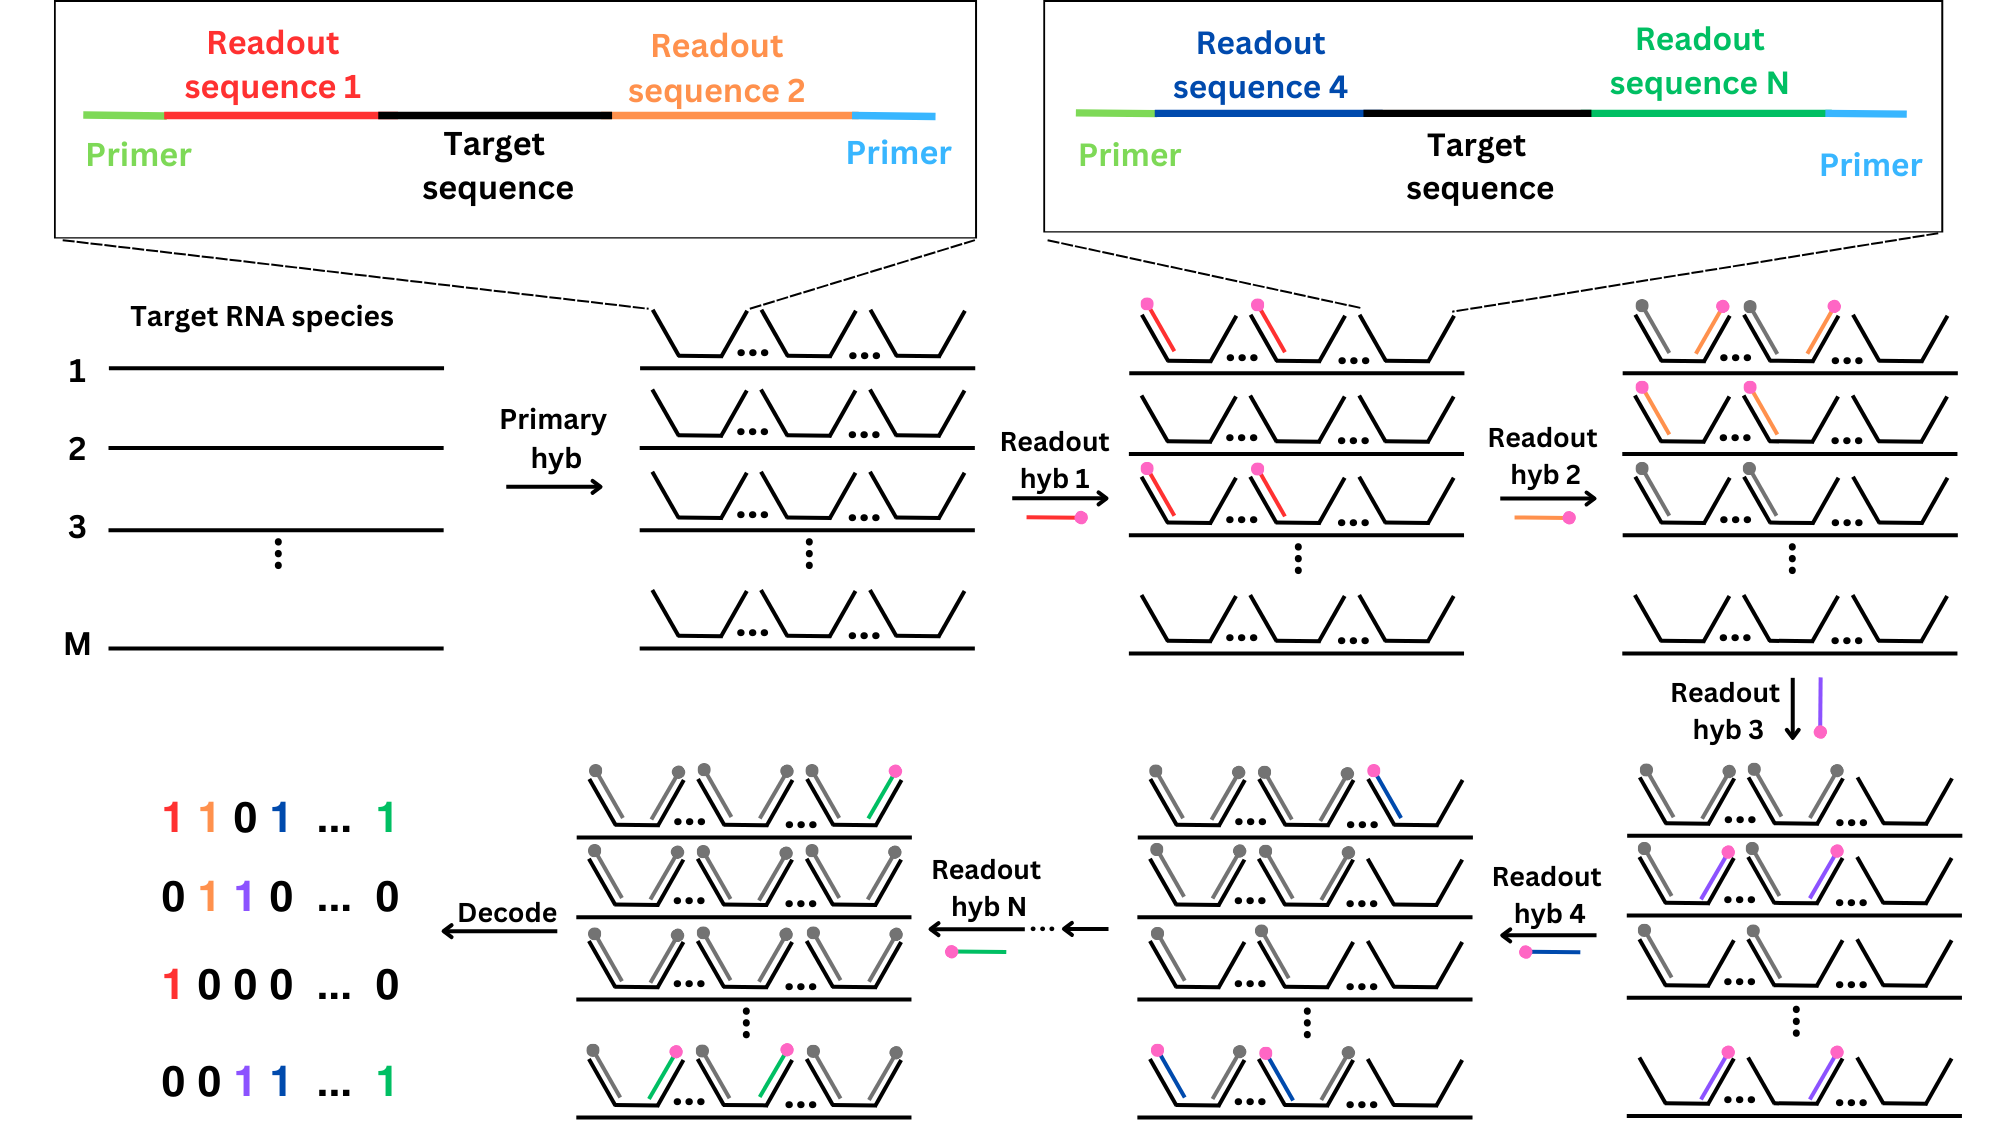
\includegraphics[width=\linewidth]{main_thesis/figure/1A.png} 
        \label{fig1A}
    \end{subfigure}
    \begin{subfigure}[t]{0.45\textwidth}
            \caption{}
            \centering
            \label{fig1B}
            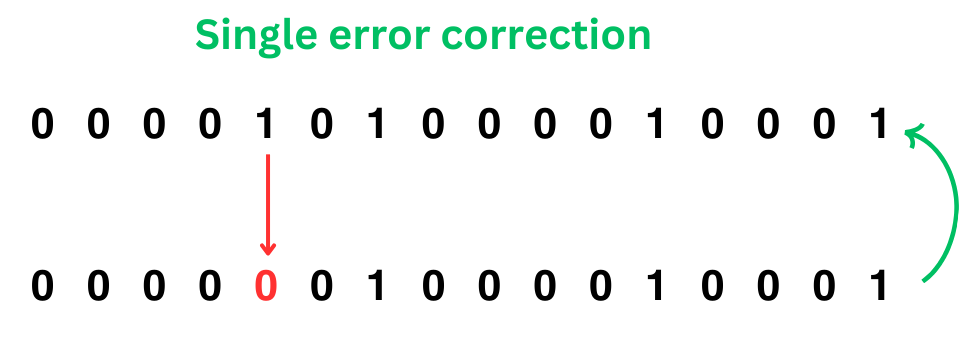
\includegraphics[width=\linewidth]{main_thesis/figure/1B.png} 
            
    \end{subfigure}
    \begin{subfigure}[t]{0.45\textwidth}
        \centering
        \caption{}
        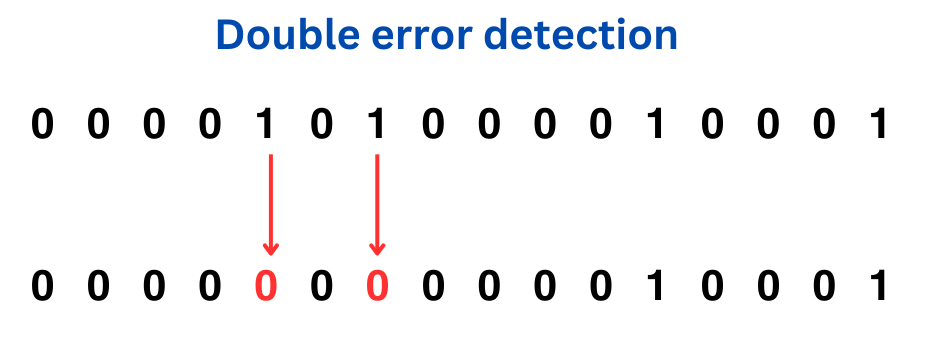
\includegraphics[width=\linewidth]{main_thesis/figure/1C.png} 
        \label{fig1C}
    \end{subfigure}
    
    \caption{\textbf{MERFISH: A highly multiplexed smFISH approach enabled by combinatorial labelling and error-robust encoding.} (\textbf{\subref{fig1A}}) Schematic of MERFISH. Every RNA species has an N-bit binary code encoded, and only a subset of RNAs should read 1 in the corresponding bit emit signal during each imaging round. First, each species of RNA has labelled target probes, which change the RNA into a particular set of readout sequences (primary hybridisation). The central RNA-targeting region of these encoding probes is flanked by readout sequences selected from a pool of N distinct sequences, each connected to a distinct hybridisation round. N consecutive rounds of hybridisation (hyb) with the fluorescent readout probes are used to probe the readout sequences (hyb 1, hyb 2,..., hyb N). Encoding probes for a particular RNA species contain a specific combination of four N readout sequences, corresponding to the four hybridisation rounds in which this RNA should read 1. To prevent them from interfering in later steps, the readout probes will be deactivated using photobleaching between each round of adding new probes. The illustration only shows one example of how the readout sequences might pair up. In reality, all four possible combinations of these sequences are used equally and scattered randomly across each RNA molecule in the experiment.  (\textbf{\subref{fig1B}}-\textbf{\subref{fig1C}})Schematic showing how an encoding scheme with a Hamming distance of 4 can detect and correct single-bit errors but can only detect double-bit errors.}
\end{figure}
\pagebreak
\noindent Here, I classified microbes from metagenomics data collected from lung samples \parencite{campos-2023}. The readout probe design was done using PaintSHOP, and the resulting probe library went through quality control to achieve higher accuracy. I also designed readout sequences, readout probes for the fluorescence hybridisation process, and primers to amplify the probes. This work aims to develop a pipeline to design probes for MERFISH experiments to obtain the spatial information of microbial communities in human lung cells.
%%%%%%%%%
%%%%%%%%%
%%%%%%%%% MATERIAL & METHODS
%%%%%%%%%
%%%%%%%%%

\section*{Materials and methods}
%%%%%
\subsection*{Classification of microbes and abundance estimation}
The data used in this research came from previously sampled and sequenced from active, former, and never smokers. The sampling included 55 volunteer subjects who are over 40 years old, either nonsmokers or smokers with at least ten pack-years of smoking history. Exclusion criteria included pulmonary malignancies, recent antibiotic or steroid use, chronic lung conditions, and acute respiratory infections. Subjects underwent bronchoscopy for bronchoalveolar lavage fluid collection, followed by DNA extraction, purification, and sequencing to obtain the metagenomic DNA \parencite{campos-2023}. 

\noindent Kraken2 (v2.1.2)\parencite{wood-2019} is a widely-used bioinformatics tool for classifying DNA sequences based on their taxonomic origin. It compares input sequences to a reference genome database and assigns them taxonomic labels. Bracken (v2.8)\parencite{alam-2017} complements Kraken2 by estimating taxon abundance in metagenomic samples, utilising Kraken2's output for more precise estimates. This integration enhances taxonomic and abundance information accuracy. Metagenomic analysis using the Kraken2 pipeline (Nguyen, unpublished) was conducted to examine the microbial sequences present in the metagenomic data. 

\noindent In short, the metagenomic data went through raw data processing with Trimmomatic (v0.39)\parencite{bolger-2014}. This tool was designed to remove low-quality reads, adapter sequences, and other contaminants to improve the quality of sequencing data. The trimmed data was then going through quality control with FastQC (v0.12.1)\parencite{Andrews:2010tn} and summarised with MultiQC (v1.21)\parencite{ewels-2016} for future decision-making. Next, Kraken2 was run on the trimmed data to classify microbes with the default parameters; the references database for the classification process was a pre-compiled Refseq database of archaea, bacteria, viral, plasmid, UniVec Core (sources of sequencing contamination), protozoa, fungi and human as the representative metazoan (PlusPF database, last updated 12/9/2022). Finally, Bracken was run on Kraken2’s reports to obtain the list of different taxa. The analysis specifically quantified reads at the species level, counting only species supported by ten or more reads.
%%%%%
%%%%%
\subsection*{Raw data processing}
A list of microbes species was obtained after the classification. NCBI command line tools (v16.3.0)\parencite{ncbi2024} help to gather data from across NCBI databases quickly. The downloaded data are sequence files in FASTA format and their GTF annotation file, limited to the latest annotated reference genomes from RefSeq at the complete assembly level. Species that have not been classified at the species level were excluded. 
%%%%%
%%%%%
\subsection*{Probe design}
Theoretically, every species classified from the data was randomly assigned to one of the 16-bit MHD4 code’s 140 binary codes, adapted from La Jolla Covering Repository Tables \parencite{gordon2024lajolla}. 16-bit refers to the number of rounds of hybridisation, MHD4 code refers to modified hamming distance 4 code, where the hamming distance between each code is equal or greater than 4, and the number of 1 bits is kept at four.

\noindent The template molecule for each encoding probe is made up of three components: (i) a central targeting sequence used for in situ hybridisation with the target RNA, (ii) three flanking readout sequences that hybridise with three distinct readout probes, and (iii) two flanking primer sequences that enable enzymatic amplification of the probes (Fig.~\ref{fig2}).
\newline
\begin{figure}[H] %% usepackage{float} and H for it doesnt stay on top
    \centering
    \caption{\textbf{Oligo probe composition.} Every oligo probe sequence designed with this pipeline will have a central target region that can bind to target RNA, three flanking readout sequences, and two flanking index primers.}
    \centering
    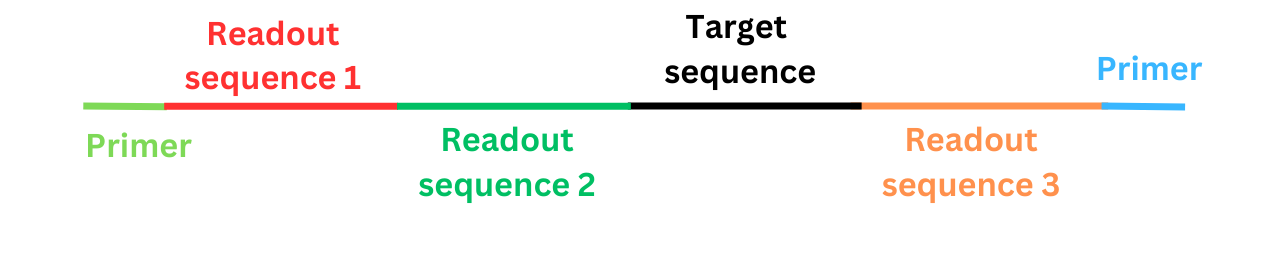
\includegraphics[width=\linewidth]{main_thesis/figure/2.png} 
    \label{fig2}
\end{figure}
%%%
\subsubsection*{Targeting probes design with PaintSHOP}
In the targeting probes design phase, deep analysis is applied by algorithms to find new probes to the sequence data of an assembled genome \parencite{beliveau-2018}. These algorithms, which include several probe designing tools such as OligoArray \parencite{rouillard-2003}, OligoPicker \parencite{wang-2003}, OligoMiner \parencite{beliveau-2018}, carefully examine sequence attributes like length, GC content, melting temperatures (Tm), and structural characteristics to find specified probe sequences. They also consider the formation of secondary structures and homopolymeric runs, two possible undesirable sequence features. This serves as the foundation for probe selection.

\noindent The Paint Server and Homology Optimization Pipeline (Hershberg et al., 2021), or PaintSHOP, serves as a modern computational platform that enables researchers to easily design oligo-based Fluorescence In Situ Hybridisation (FISH) experiments at the transcriptome and genome scales. PaintSHOP consists of two main parts: a bioinformatic pipeline and an interactive web application. While the interactive web application offers all facets of constructing the probe set, it only provides them within some of its pre-existing collections. Therefore, the target sequences were designed using the bioinformatic pipeline from PaintSHOP.

\noindent The PaintSHOP pipeline takes the FASTA sequence and GTF gene annotations file as input for a genome assembly. In detail, it begins with parsing the genome data and constructing the Jellyfish k-mer database. Probes are then designed for all chromosomes, both DNA and RNA targets, with the given Tm and the desired length of the probe, followed by building a Bowtie index for these probes. The designed probes are aligned using Bowtie, and SAM files are converted to pairwise alignment format while extracting alignment scores. The pairwise alignment data is parsed, and duplex structures are predicted. The designed probes are then scored. Probes are filtered, and the maximum k-mer occurrences are determined. Further filtering of probes and calculation of maximum k-mer values are performed. The GTF file is parsed for annotation, and probe data is merged. A reference sequence database is generated, and the probe data is compressed. The workflow concludes with the finalisation of these processes. The Tm and the probes’ length for the run were set at 42 degree C and 30-nucleotide (nt) respectively.

% Isoforms are flattened for each chromosome, and the flattened annotations are merged.

\noindent To eliminate potentially off-binding probes, a filtering step was implemented using BLAST+ (v2.15.0) \parencite{camacho-2009}. I specified that probes for one species with 15 or more bases of homology on other species were removed, keeping only the probes mapped to their species. To further improve specificity, the probes were screened against the human genome. Probes that could be mapped to the human genome with a minimum homology of 15 bases are eliminated. 

\noindent Finally, to specifically select RNA probes, the probes’ location was compared against the annotation file to find probes that were produced to land on the coding region. Additionally, any probe that have high off-target score evaluated with PaintSHOP was removed. For each species, a minimum of 20 and a maximum of 50 probes were selected. Any species which fell to have at least 20 target probes were eliminated.
%%%
\subsubsection*{Readout sequences design}
A large pool of random sequences was generated to create readout sequences. These sequences were 20-nt long, with a roughly equal probability of 25\% of A and T and 50\% of G. Importantly, sequences with stretches of Gs longer than three nucleotides were excluded. This step prevents the formation of G-quadruplex structures, which can hinder synthesis and binding processes.
To reduce the vast number of generated sequences, BLAST+ was employed to identify and remove those with excessive similarity (cross-homology) to the human transcriptome and the genomes of classified lung microbes. This step required high-performance computing (HPC) since millions of possible readout sequences needed to be evaluated if they have off-target or not. A threshold of 11 contiguous matching bases was used for the human transcriptome, while a threshold of 12 was used for lung microbes. This distinction was necessary because a threshold of 11 for lung microbes would have eliminated all remaining sequences after filtering against the human transcriptome. Finally, the remaining sequences underwent an additional screening step to ensure they exhibited minimal similarity (no more than 11-nt) to each other \parencite{chen-2015}. These readout sequences were probed, one in each hybridisation round, using fluorescently labelled readout probes containing sequences complementary to the readout sequences. 

%%%
\subsubsection*{Primers design}
The designed oligo probes will be amplified through PCR. Primer sequences for this experiment were produced from a set of 25-nt orthogonal sequences \parencite{xu-2009}. These sequences were randomly trimmed to 20-nt and were filtered to have (i) a narrow range of Tm from 59-60 degrees C, (ii) no stretches of C or G longer than three bases, (iii) a GC clamp which refers to the presence of G or C at the tail end, (iv) low Tm of hairpin formation and self-dimerisation, (v) a GC content from 35-65\%. These primers were further screened with homology threshold was 11-nt and 12-nt or more were removed against human transcriptome and microbes' genome respectively, using BLAST+. 


%%% A final screening step against T7 promoter was also performed to add it to the selected reverse primer, allowing \textit{in vitro} transcription.
%%%%%
%%%%%
%%%%% RESULT
%%%%%
%%%%%
\section*{Results}
The flow chart of the pipeline of this research is summarised in Fig.~\ref{fig3}. In brief, the pipeline involves four steps involving the design of (i) codebook, (ii) target sequence, (iii) readout sequences, readout probes and (iv) primers. The codebook is important as it decides the number of readout sequences needed to be generated; for instance, this pipeline uses 16-bit, which means 16 different readout sequences and readout probes are required. La Jolla tables provided a wide range of covering tables that can be adapted to design the codebook depending on the round, the hamming distance, and the hamming weight. For this 16-bit HMD4, the table C(16,4,3) was used. The microbes needed to be classified from metagenomic data using the Kraken2-Bracken pipeline to design the target sequence. After having the microbes list, their genome file and annotation file were downloaded using the NCBI command line tool. Target probes can now be designed with PaintSHOP and go through screening steps against other microbes and the human genome. After that, the probes were filtered again to obtain RNA probes with low off-target score, then 20 to 50 target probes were selected for each species. Readout sequences were designed by generating a pool of oligonucleotide sequences with a length of 20 with A, T and G. These were filtered down by screening against the human genome and microbes with the help of HPC. They were screened against themselves to obtain 16 orthogonal sequences (Table~\ref{table1}). The 20-nt primers were designed from a set of 25-nt orthogonal sequences, which were trimmed and went through quality control to obtain 2 suitable primers (Table~\ref{table2}). Finally, all those components were combined into a table, with over 4300 encoding probes for all species. Details on how to apply the pipeline can be found through \url{https://github.com/npxhuy/MERFISH_probeDesign}.

%%TABLE1
\begin{table}[H]
\caption{{\bf All used readout sequences.}}
\begin{tabular}{|l|l|}
\hline
\textbf{Bit} & \textbf{Readout sequence} \\ \hline
1            & AGATTAGGAGGGTAGTTATG      \\ \hline
2            & AATAGTAGGGTGGTAGTTGG      \\ \hline
3            & TGTATAGAGTAAGGGATGTG      \\ \hline
4            & TGATATAGTGGGAGTAAGGT      \\ \hline
5            & AGAGGATTAGTGTGGAGTAG      \\ \hline
6            & GGTGTGTGTGTGTAAGAAGA      \\ \hline
7            & TAGGGAGTTATAGGTAGGGA      \\ \hline
8            & AGATGGATAGGGTTATGAGT      \\ \hline
9            & GTGTAAGAGTGGTAGGTAGG      \\ \hline
10           & AGATGTAGGTTAGGTGAGAG      \\ \hline
11           & GGTTAGAGAGAGAGAGGTTT      \\ \hline
12           & ATAGTGAGTAGTGGGTTAAG      \\ \hline
13           & ATTGATAGGGAGGTTAGATG      \\ \hline
14           & AGGGTATAGTTAGAGTGTAG      \\ \hline
15           & GTTAGAGAGAGAGAGGGTTT      \\ \hline
16           & TGAAAGGGTGTAGTATATGG      \\ \hline
\end{tabular}
\label{table1}
\end{table}
%%END TABLE1

\begin{figure}[H]
    \centering
    \caption{\textbf{Flow chart of the pipeline} of oligo probes designed for MERFISH on microbes in a particular organ given the metagenomic data. Details on how to apply the pipeline can be found through \url{https://github.com/npxhuy/MERFISH_probeDesign}}
    \centering
    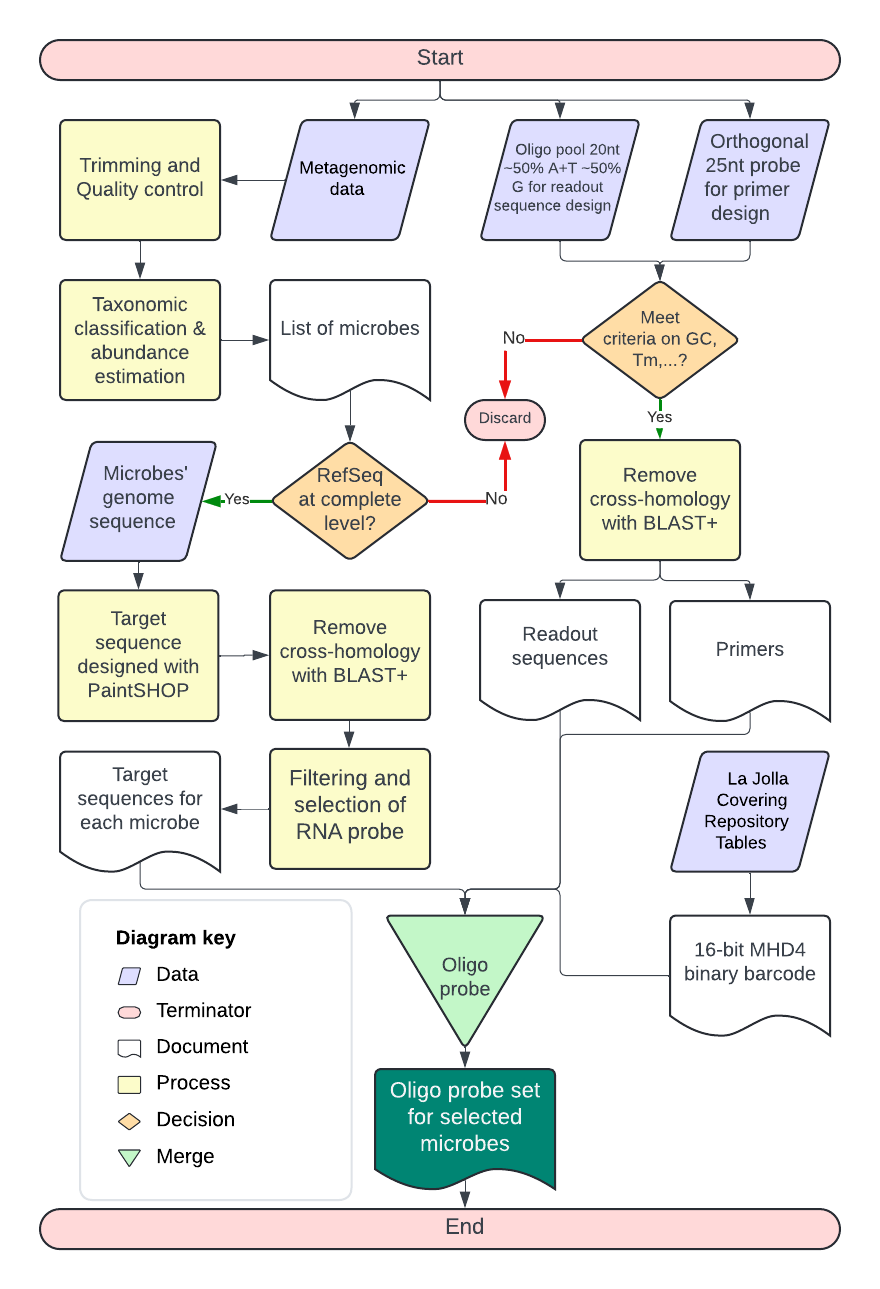
\includegraphics[width=\linewidth]{main_thesis/figure/3.png} 
    \label{fig3}
\end{figure}
\pagebreak




%%TABLE2
% AGACGCGGGAGCTAGCTGTC
% TCGGCAAGAGACCCGCTCAA
% T7 + rev-comp TAATACGACTCACTATAGGG TTGAGCGGGTCTCTTGCCGA
% Forward primer
% Reverse primer with T7 promoter
\begin{table}[H]
\caption{{\bf All used primer sequences.}}
\begin{tabular}{|l|l|}
\hline
\textbf{}        & \textbf{Primer sequences} \\ \hline
\textbf{Forward} & CGTGTTAGTGGCCCGGGTCT      \\ \hline
\textbf{Reverse} & GGCCGCGACTAGGTAAGCCT      \\ \hline
\end{tabular}
\label{table2}
\end{table}



\noindent The classification of microbes with Kraken2 and abundance estimation with Bracken identify  153 classified species. I precisely wanted to have microbes that have their annotated genome data at the complete assembly level from RefSeq, and 97 species met this requirement (Table~\ref{tableS1}).

\noindent The number of DNA probes generated by PaintSHOP varies from species to species. Some species had over 170000 candidate probes without filtering, while others had less than 3000. This could be explained as some species have smaller genomes than others, thus there are fewer probes that fit the length and Tm. After filtering steps against other species and the human genome, the number of probes decreased dramatically, where some species had no available probes as their candidate probes have off-target (Table~\ref{tableS1}). Since the minimum threshold of the number of probes was 20 probes per species, some species were discarded. Species that achieved the threshold were assigned randomly with a unique binary 16-bit MHD4 barcode (Table ~\ref{tableS2}). The full encoding table is available at \url{https://github.com/npxhuy/MERFISH_probeDesign/blob/main/probe_table.tsv}, Table ~\ref{tableS3} shows the first 5 lines of the final probes table.

%%%%%
%%%%%
%%%%% DISCUSSION
%%%%%
%%%%%
\section*{Discussion}
Numerous human organs contain microbial communities, and unveiling the complex spatial distribution of these microbial communities can provide valued understanding through spatial transcriptomics techniques. Here, we describe a potent workflow for determining the spatial distribution of microbes in lung tissue sections using a thoughtfully constructed MERFISH probe table.

\noindent The probe table is the foundation for future MERFISH experiments on human lung microbes. Companies specialising in oligonucleotide synthesis can be readily contacted to generate the desired probes based on the provided sequences. Notably, in-house amplification is made possible by the primers included in the probe table. Especially for large-scale studies, this amplification capability enables researchers to obtain larger quantities of probes at a lower cost than repeat vendor orders.

\noindent This workflow can be extended to investigate microbial communities within other human tissues. By designing probes targeting specific microbial RNA sequences relevant to the tissue of interest, researchers can gain valuable insights into the spatial distribution of microbes in the gut, skin, or any other tissue harbouring a resident microbiome. This adaptability makes the design of the MERFISH probe table workflow a solid pipeline for various microbiome research endeavours.

\noindent The MERFISH experiment can begin after the required probes are obtained by in-house amplification or vendor synthesis. In this experiment, the probes are hybridised to the target RNA in the tissue section, and then detection and image analysis are performed. The experiment's outcome offers a high-resolution map of the tissue's microbial communities, illuminating their spatial arrangement and possible interactions.

\noindent While MERFISH is a powerful technique, it's not without limitations with two potential error sources: missing some RNA molecules (undercounting) and misidentifying RNA from one species for another. However, these errors appear infrequent. Research on this technique developed methods to assess misidentification rates and estimate the success rate of RNA detection (calling rate). It found that over 90\% of RNA species showed high confidence in identification, and the calling rate was estimated to be around 80\% \parencite{chen-2015}. The validation steps demonstrated high concordance with MERFISH results, which employed various codebooks, a comparison with other techniques (smFISH), bias in measurements, estimation of calling rate, and bulk RNA sequencing data. This implies that MERFISH is a reliable method, successfully detects RNA molecules, producing accurate gene expression data despite potential errors. 

\noindent The metagenomic data was sequenced using the 454 sequencing technique \parencite{campos-2023}. While Trimmomatic is primarily designed to handle Illumina data, it can still be effective for adapter trimming in this context. Given the lack of specific adapter information, the standard Trimmomatic settings were employed for adapter removal. FastQC reports demonstrate a clear improvement in sequence quality after this step (Fig.~\ref{fig1SA}-~\ref{fig1SB}). Consequently, the trimmed data generated by Trimmomatic was used for downstream analyses like taxonomic classification and abundance estimation.

\noindent PaintSHOP's target probe design pipeline can also generate RNA probes. However, none of the RNA probes passed the filter during the initial filtering step, which was designed to limit off-target binding. Due to this lack of suitable RNA probes, DNA probes were chosen instead. These DNA probes were then filtered to ensure they would target the coding regions of the microbes of interest.

\noindent The amplification of encoding probes for target RNA detection in MERFISH is an important step to achieve a good concentration before the encoding probes staining process, for example around 1 nM for a (tissue) sample volume of 25 \ensuremath{\mu}L \parencite{xia-2019}. While traditional PCR offers a robust and well-established method for probe amplification, it can introduce unwanted bias \parencite{polz-1998}. This bias arises because PCR amplification efficiency can vary depending on the target sequence or strength of primer binding, leading to some being amplified more efficiently than others. Isothermal amplification methods like Multiple Displacement Amplification (MDA) emerge as a good alternative with less bias \parencite{spits-2006}\parencite{zanoli-2012}. 


\noindent Photobleaching is an essential stage in the MERFISH imaging process to detect multiplexed probes precisely by removing signal interference from earlier rounds. A persistent loss of fluorescence signal results from photobleaching, which reduces observation time and spatiotemporal resolution. Using bioorthogonal cleavable fluorescent oligonucleotides for highly multiplexed single-cell in situ RNA and DNA analysis offers a potentially effective substitute for photobleaching. This method uses a chemically cleavable linker to bind oligonucleotide probes to fluorophores. Without affecting the integrity of the target nucleic acids, the fluorophores can be effectively cleaved off at 37°C in 30 minutes following hybridisation and imaging. By removing the fluorescent signal, this chemical cleavage eliminates the need for photobleaching and all of its adverse effects, including phototoxicity and irreversible signal loss. The hybridised probes are subsequently removed to facilitate the hybridisation of the next set of probes for the ensuing imaging cycle \parencite{mondal-2018}.
%%%%%
%%%%%
%%%%% ACK
%%%%%
%%%%%
\section*{Acknowledgments}
I would like to express my sincere gratitude to my supervisor, Dr. Nils Norlin, from the Department of Experimental Medical Science, for his invaluable guidance and support throughout my project. Dr. Norlin's expertise, patience, and dedication have shaped my research journey. His insightful feedback and constructive criticism have consistently pushed me to exceed my expectations. I am truly fortunate to have him as my supervisor, and I am grateful for the opportunity to learn from his vast knowledge and experience. Thank you, Dr. Norlin, for your unwavering encouragement and for being an exceptional mentor. Computations and analyses were enabled by resources provided by the National Academic Infrastructure for Supercomputing in Sweden (NAISS), partially funded by the Swedish Research Council through grant agreement no. 2022-06725. Finally, I would like to send my kind love to my family, who supported me greatly during my time here. Cam on bo me \& chi Quynh.
\nolinenumbers

% Reference
\printbibliography
\newpage
\section*{Supporting information}


\subsection*{Supplementary figures}
\beginsupplement{

\renewcommand\thesubfigure{\Alph{subfigure}} % Make subfigure labels uppercase
\begin{figure}[H]
    \centering
    \begin{subfigure}[t]{0.45\textwidth}
            \caption{}
            \centering
            \label{fig1SA}
            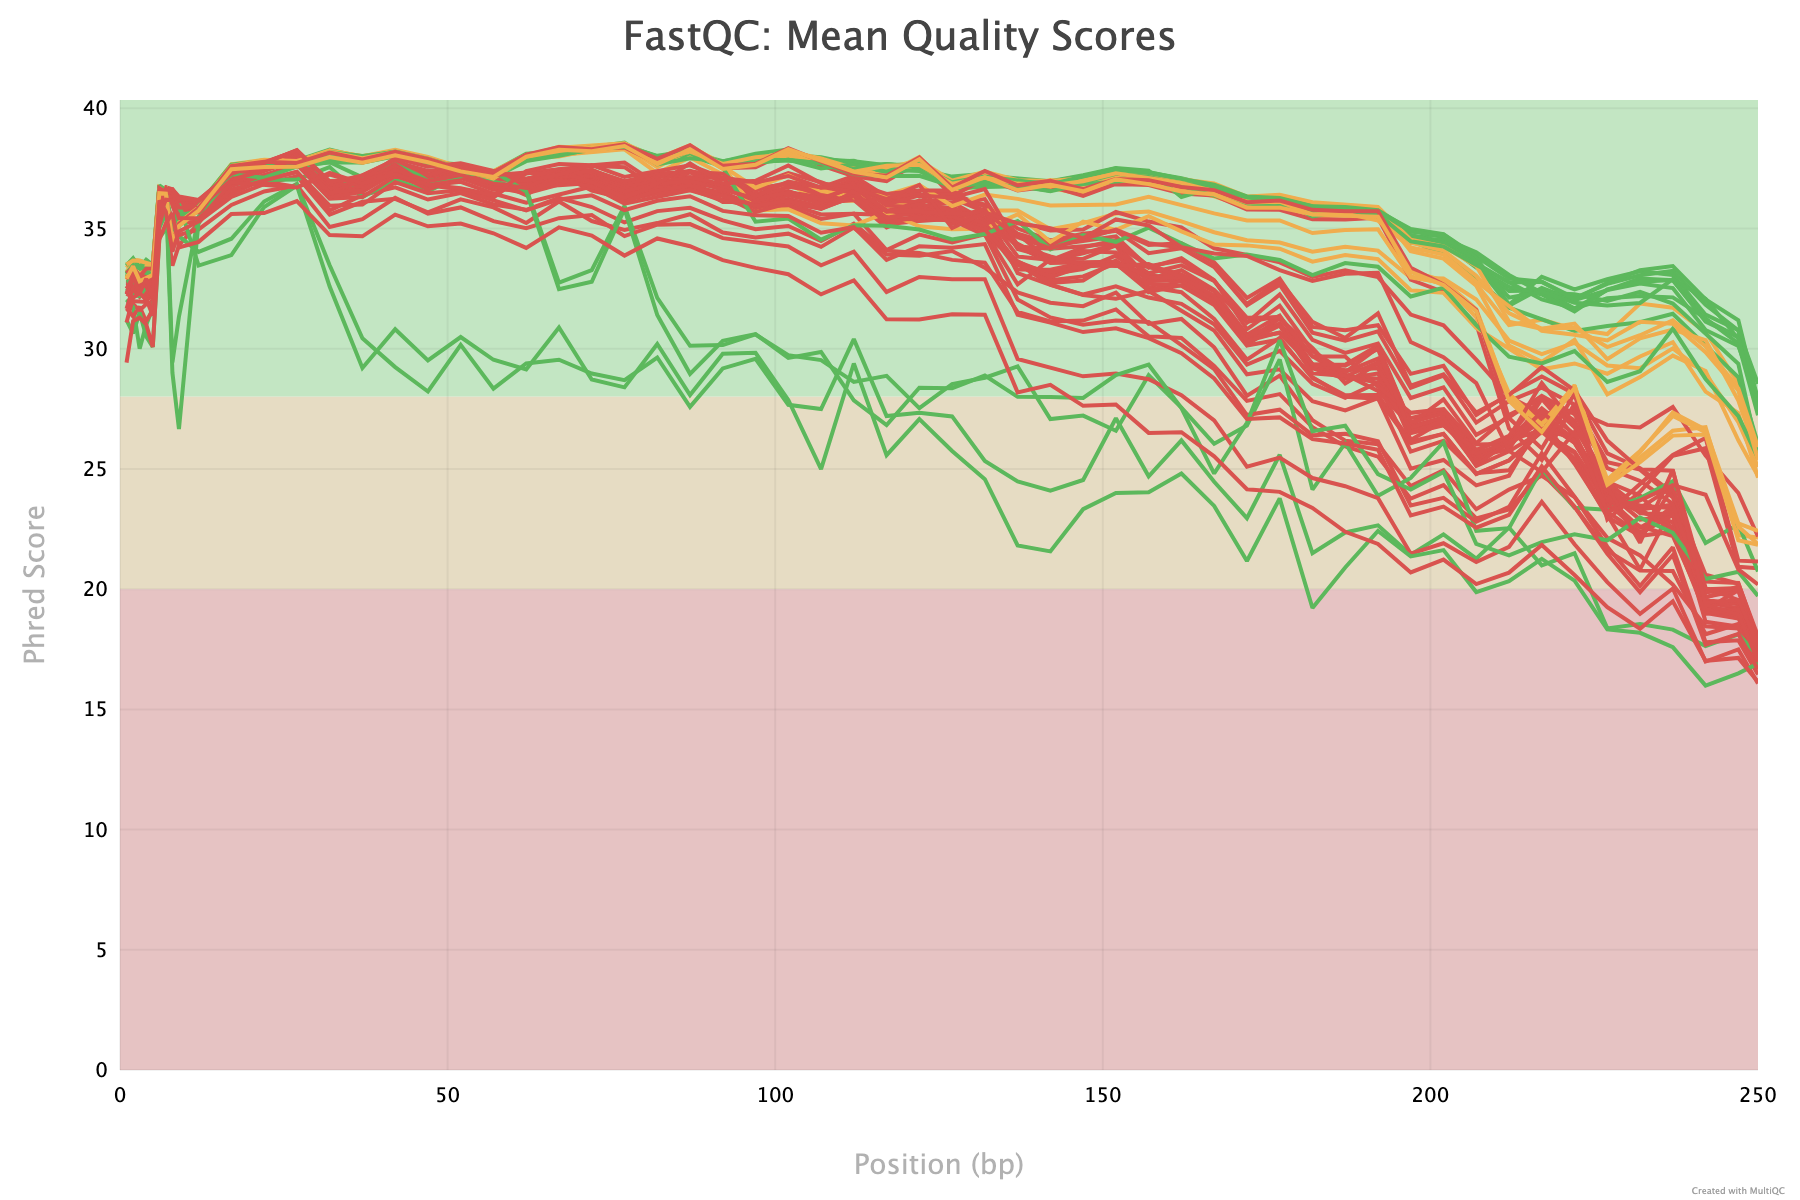
\includegraphics[width=\linewidth]{main_thesis/figure/1SA.png} 
            
    \end{subfigure}
    \begin{subfigure}[t]{0.45\textwidth}
        \centering
        \caption{}
        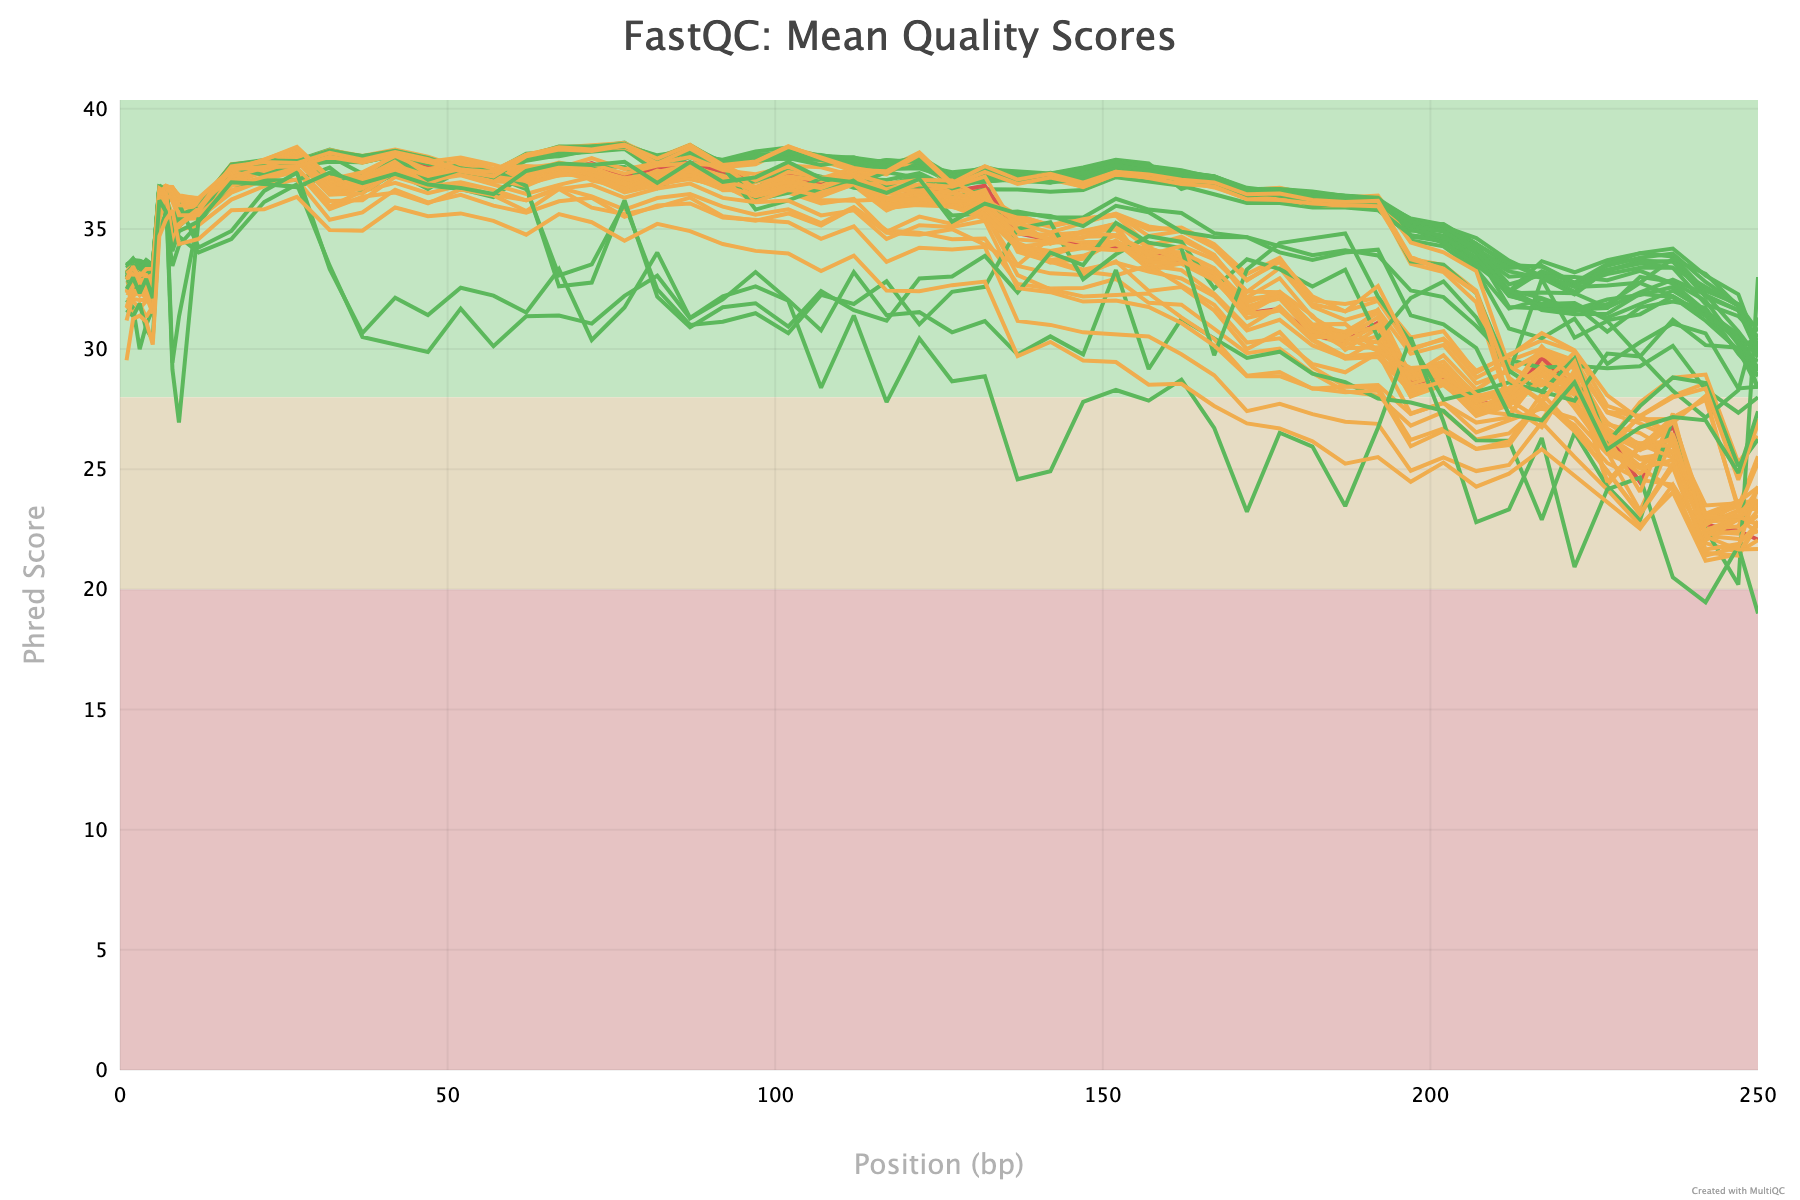
\includegraphics[width=\linewidth]{main_thesis/figure/1SB.png} 
        \label{fig1SB}
    \end{subfigure}
    
    \caption{\textbf{MultiQC report of mean quality score} of \subref{fig1SA} raw sequencing data and \subref{fig1SB} trimmed data with Trimmomatic. This graph depicts the average Phred quality score across each base position in the sequencing reads. Phred scores represent the accuracy of base calls, with higher scores indicating better quality. Each line shows the average Phred score at each base position across all samples—a line hovering mainly in the green zone, indicating good quality across all bases. If a significant portion of the line falls into the orange or red zones, it suggests lower-quality reads that might require further investigation.}
\end{figure}


}
\newpage
\subsection*{Supplementary tables}
\beginsupplement{
\begin{longtable}
{| p{.50\textwidth} | p{.20\textwidth} | p{.20\textwidth} |} 
\caption{\textbf{List of classified species and their number of probes} generated by PaintSHOP and after filtering} % needs to go inside longtable environment
\label{tableS1}
\hline
\textbf{Species}                               & \textbf{Candidated probes}      & \textbf{Filtered}   \\ \hline
Acinetobacter baumannii               & 56618  & 193 \\ \hline
Actinopolyspora erythraea             & 171406 & 333 \\ \hline
Agathobacter rectalis                 & 64754  & 102 \\ \hline
Anaerococcus mediterraneensis         & 12812  & 36  \\ \hline
Aquirhabdus parva                     & 115548 & 395 \\ \hline
Bacillus cereus                       & 39148  & 152 \\ \hline
Bacillus spizizenii                   & 102070 & 176 \\ \hline
Bacillus velezensis                   & 125358 & 239 \\ \hline
Bifidobacterium adolescentis          & 107964 & 151 \\ \hline
Bifidobacterium longum                & 115920 & 153 \\ \hline
Blautia argi                          & 63568  & 77  \\ \hline
Blautia obeum                         & 64924  & 85  \\ \hline
Blautia wexlerae                      & 83124  & 123 \\ \hline
Burkholderia mallei                   & 181456 & 210 \\ \hline
Candidatus Desulforudis audaxviator   & 96170  & 170 \\ \hline
Candidatus Mycosynbacter amalyticus   & 43370  & 210 \\ \hline
Candidatus Nanosynbacter lyticus      & 19066  & 76  \\ \hline
Candidatus Saccharimonas aalborgensis & 34834  & 169 \\ \hline
Capnocytophaga leadbetteri            & 39532  & 207 \\ \hline
Capnocytophaga sputigena              & 36874  & 146 \\ \hline
Cardiobacterium hominis               & 116030 & 119 \\ \hline
Changpingibacter yushuensis           & 140384 & 469 \\ \hline
Coprococcus comes                     & 67524  & 95  \\ \hline
Coprothermobacter proteolyticus       & 33138  & 108 \\ \hline
Corynebacterium durum                 & 134344 & 362 \\ \hline
Corynebacterium glucuronolyticum      & 141548 & 398 \\ \hline
Corynebacterium macginleyi            & 116868 & 363 \\ \hline
Corynebacterium suedekumii            & 106028 & 127 \\ \hline
Cutibacterium acnes                   & 133986 & 304 \\ \hline
Cutibacterium granulosum              & 102274 & 138 \\ \hline
Cutibacterium modestum                & 138762 & 364 \\ \hline
Deinococcus geothermalis              & 123528 & 159 \\ \hline
Dermabacter vaginalis                 & 115708 & 291 \\ \hline
Filifactor alocis                     & 12970  & 30  \\ \hline
Finegoldia magna                      & 6452   & 15  \\ \hline
Fusobacterium animalis                & 2490   & 0   \\ \hline
Fusobacterium hwasookii               & 2580   & 1   \\ \hline
Fusobacterium polymorphum             & 2492   & 1   \\ \hline
Fusobacterium pseudoperiodonticum     & 2784   & 1   \\ \hline
Fusobacterium vincentii               & 2350   & 0   \\ \hline
Gemella haemolysans                   & 5112   & 9   \\ \hline
Gemella morbillorum                   & 5554   & 15  \\ \hline
Gemella sanguinis                     & 4142   & 12  \\ \hline
Haemophilus parahaemolyticus          & 36772  & 133 \\ \hline
Hoylesella buccalis                   & 94050  & 216 \\ \hline
Hoylesella enoeca                     & 90288  & 274 \\ \hline
Klebsiella michiganensis              & 268780 & 610 \\ \hline
Lacticaseibacillus paracasei          & 95928  & 310 \\ \hline
Lancefieldella parvula                & 42548  & 152 \\ \hline
Leptotrichia buccalis                 & 8180   & 13  \\ \hline
Leptotrichia wadei                    & 7660   & 7   \\ \hline
Megasphaera stantonii                 & 108414 & 215 \\ \hline
Methylobacterium organophilum         & 161248 & 181 \\ \hline
Mogibacterium diversum                & 27834  & 128 \\ \hline
Mycobacterium spongiae                & 235684 & 610 \\ \hline
Neisseria elongata                    & 101754 & 125 \\ \hline
Olsenella uli                         & 88828  & 159 \\ \hline
Parvimonas micra                      & 3632   & 4   \\ \hline
Peptoniphilus equinus                 & 50654  & 159 \\ \hline
Prevotella dentalis                   & 142872 & 167 \\ \hline
Prevotella denticola                  & 119082 & 108 \\ \hline
Prevotella histicola                  & 47850  & 110 \\ \hline
Prevotella jejuni                     & 66340  & 189 \\ \hline
Prevotella melaninogenica             & 48900  & 76  \\ \hline
Prevotella multiformis                & 123020 & 123 \\ \hline
Prevotella nigrescens                 & 64470  & 172 \\ \hline
Propionibacterium acidifaciens        & 85518  & 74  \\ \hline
Propioniciclava coleopterorum         & 90626  & 80  \\ \hline
Roseburia intestinalis                & 96220  & 150 \\ \hline
Schaalia meyeri                       & 83242  & 169 \\ \hline
Segatella oris                        & 78936  & 180 \\ \hline
Selenomonas dianae                    & 108258 & 175 \\ \hline
Selenomonas sputigena                 & 117464 & 151 \\ \hline
Slackia heliotrinireducens            & 153154 & 237 \\ \hline
Staphylococcus aureus                 & 12166  & 39  \\ \hline
Staphylococcus epidermidis            & 9290   & 26  \\ \hline
Stenotrophomonas maltophilia          & 168314 & 59  \\ \hline
Stenotrophomonas pavanii              & 166214 & 92  \\ \hline
Streptococcus agalactiae              & 13888  & 27  \\ \hline
Streptococcus anginosus               & 24808  & 52  \\ \hline
Streptococcus cristatus               & 41944  & 84  \\ \hline
Streptococcus gordonii                & 33608  & 64  \\ \hline
Streptococcus mutans                  & 19454  & 31  \\ \hline
Streptococcus oralis                  & 31008  & 72  \\ \hline
Streptococcus parasuis                & 30240  & 65  \\ \hline
Streptococcus pyogenes                & 19214  & 49  \\ \hline
Streptococcus sanguinis               & 53916  & 82  \\ \hline
Streptococcus suis                    & 34870  & 54  \\ \hline
Streptococcus thermophilus            & 19996  & 53  \\ \hline
Streptococcus urinalis                & 10806  & 21  \\ \hline
Subdoligranulum variabile             & 138224 & 119 \\ \hline
Tannerella forsythia                  & 109956 & 389 \\ \hline
Treponema socranskii                  & 106074 & 257 \\ \hline
Tropheryma whipplei                   & 26446  & 131 \\ \hline
Trueperella pyogenes                  & 113430 & 269 \\ \hline
Veillonella rodentium                 & 48052  & 197 \\ \hline
Xanthomonas albilineans               & 166178 & 266 \\ \hline

\end{longtable}

\begin{longtable}
{| p{.50\textwidth} | p{.40\textwidth} |} 
\caption{\textbf{List of species and their binary MH4D barcode.} Species that did not have enough probes after the filtering step were discarded.} % needs to go inside longtable environment
\label{tableS2}
\hline
\hline
\textbf{Species}                      & \textbf{Binary barcode} \\ \hline
Acinetobacter baumannii               & 1000000101000010        \\ \hline
Actinopolyspora erythraea             & 1100000000001100        \\ \hline
Agathobacter rectalis                 & 0010100000010100        \\ \hline
Anaerococcus mediterraneensis         & 1001000001100000        \\ \hline
Aquirhabdus parva                     & 0001010001000001        \\ \hline
Bacillus cereus                       & 1100110000000000        \\ \hline
Bacillus spizizenii                   & 1100001100000000        \\ \hline
Bacillus velezensis                   & 0100000100010100        \\ \hline
Bifidobacterium adolescentis          & 1000000100100100        \\ \hline
Bifidobacterium longum                & 0100001001000010        \\ \hline
Blautia argi                          & 0000101010100000        \\ \hline
Blautia obeum                         & 0010001000100010        \\ \hline
Blautia wexlerae                      & 0101000010100000        \\ \hline
Burkholderia mallei                   & 0000100100000110        \\ \hline
Candidatus Desulforudis audaxviator   & 0100100010000100        \\ \hline
Candidatus Mycosynbacter amalyticus   & 0001000100010001        \\ \hline
Candidatus Nanosynbacter lyticus      & 0011110000000000        \\ \hline
Candidatus Saccharimonas aalborgensis & 0101010100000000        \\ \hline
Capnocytophaga leadbetteri            & 0011000011000000        \\ \hline
Capnocytophaga sputigena              & 0010001010001000        \\ \hline
Cardiobacterium hominis               & 0001100000100100        \\ \hline
Changpingibacter yushuensis           & 1010000000000101        \\ \hline
Coprococcus comes                     & 1111000000000000        \\ \hline
Coprothermobacter proteolyticus       & 0000000011001100        \\ \hline
Corynebacterium durum                 & 1010101000000000        \\ \hline
Corynebacterium glucuronolyticum      & 1000010000010010        \\ \hline
Corynebacterium macginleyi            & 1000100001000100        \\ \hline
Corynebacterium suedekumii            & 0001010000101000        \\ \hline
Cutibacterium acnes                   & 1000100000100010        \\ \hline
Cutibacterium granulosum              & 0100100000100001        \\ \hline
Cutibacterium modestum                & 0100000110000010        \\ \hline
Deinococcus geothermalis              & 0011001100000000        \\ \hline
Dermabacter vaginalis                 & 0010000100100001        \\ \hline
Filifactor alocis                     & 0000110000001100        \\ \hline
Finegoldia magna                      & 0000000001010101        \\ \hline
Gemella haemolysans                   & 0000101000001010        \\ \hline
Gemella morbillorum                   & 1100000011000000        \\ \hline
Gemella sanguinis                     & 1001000000000110        \\ \hline
Haemophilus parahaemolyticus          & 0100010000010001        \\ \hline
Hoylesella buccalis                   & 0010010001000010        \\ \hline
Hoylesella enoeca                     & 0000001111000000        \\ \hline
Klebsiella michiganensis              & 1010000001010000        \\ \hline
Lacticaseibacillus paracasei          & 0000111100000000        \\ \hline
Lancefieldella parvula                & 0000000001011010        \\ \hline
Leptotrichia buccalis                 & 0110000000001001        \\ \hline
Leptotrichia wadei                    & 1001000000001001        \\ \hline
Megasphaera stantonii                 & 0100010000100010        \\ \hline
Methylobacterium organophilum         & 0000000011000011        \\ \hline
Mogibacterium diversum                & 0000001100001100        \\ \hline
Mycobacterium spongiae                & 0000000010101010        \\ \hline
Neisseria elongata                    & 0010010010000001        \\ \hline
Olsenella uli                         & 0011000000110000        \\ \hline
Peptoniphilus equinus                 & 0010000101001000        \\ \hline
Prevotella dentalis                   & 0000000010011001        \\ \hline
Prevotella denticola                  & 0000001100000011        \\ \hline
Prevotella histicola                  & 0000010110100000        \\ \hline
Prevotella jejuni                     & 0010010000011000        \\ \hline
Prevotella melaninogenica             & 0000000001100110        \\ \hline
Prevotella multiformis                & 0101000000001010        \\ \hline
Prevotella nigrescens                 & 0001001000100001        \\ \hline
Propionibacterium acidifaciens        & 0000000000111100        \\ \hline
Propioniciclava coleopterorum         & 0100000101000001        \\ \hline
Roseburia intestinalis                & 0000100100001001        \\ \hline
Schaalia meyeri                       & 1000010000100001        \\ \hline
Segatella oris                        & 0000011001100000        \\ \hline
Selenomonas dianae                    & 0001001001001000        \\ \hline
Selenomonas sputigena                 & 1000001010000010        \\ \hline
Slackia heliotrinireducens            & 1010000010100000        \\ \hline
Staphylococcus aureus                 & 1000100010001000        \\ \hline
Staphylococcus epidermidis            & 0100000100101000        \\ \hline
Stenotrophomonas maltophilia          & 1001000010010000        \\ \hline
Stenotrophomonas pavanii              & 0001000100100010        \\ \hline
Streptococcus agalactiae              & 0000100110010000        \\ \hline
Streptococcus anginosus               & 0010100010000010        \\ \hline
Streptococcus cristatus               & 0001010000010100        \\ \hline
Streptococcus gordonii                & 0000000011110000        \\ \hline
Streptococcus mutans                  & 0101000000000101        \\ \hline
Streptococcus oralis                  & 0101000001010000        \\ \hline
Streptococcus parasuis                & 1000010010000100        \\ \hline
Streptococcus pyogenes                & 0011000000001100        \\ \hline
Streptococcus sanguinis               & 1000100000010001        \\ \hline
Streptococcus suis                    & 1001100100000000        \\ \hline
Streptococcus thermophilus            & 0100100001001000        \\ \hline
Streptococcus urinalis                & 0000010101010000        \\ \hline
Subdoligranulum variabile             & 0100001000011000        \\ \hline
Tannerella forsythia                  & 1010000000001010        \\ \hline
Treponema socranskii                  & 0000000000110011        \\ \hline
Tropheryma whipplei                   & 0100010001000100        \\ \hline
Trueperella pyogenes                  & 0010100001000001        \\ \hline
Veillonella rodentium                 & 0100100000010010        \\ \hline
Xanthomonas albilineans               & 0100001010000001        \\ \hline
\end{longtable}

\afterpage{%
    \clearpage% Flush earlier floats (otherwise order might not be correct)
    \thispagestyle{empty}% empty page style (?)
    \begin{landscape}% Landscape page
        \centering % Center table
        \captionof{table}{\textbf{The encoding probes table} first five lines. The first column indicates the species. Their encoding probes combine column Primer\_1, Readout\_1, Readout\_2, Target, Readout\_3, Readout\_4, and Primer\_2. For clarity, each sequence was separated into different columns. The chromosome where the encoding probe will land is noted in the second column.}% Add 'table' caption
\begin{adjustwidth}{-1.0in}{0in}
\label{tableS3}
\begin{tabular}{|l|l|l|l|l|l|l|l|l|}
\hline
\textbf{Species}                                                   & \textbf{Chr}                                               & \textbf{Primer\_1}                                               & \textbf{Readout\_1}                                              & \textbf{Readout\_2}                                              & \textbf{Target}                                                                & \textbf{Readout\_3}                                              & \textbf{Readout\_4}                                              & \textbf{Primer\_2}                                               \\ \hline
\begin{tabular}[c]{@{}l@{}}Acinetobacter\\ baumannii\end{tabular} & \begin{tabular}[c]{@{}l@{}}NZ\_CP0-\\ 43953.1\end{tabular} & \begin{tabular}[c]{@{}l@{}}CGTGTTAGTG-\\ GCCCGGGTCT\end{tabular} &                                                                  & \begin{tabular}[c]{@{}l@{}}AGATGGATAG-\\ GGTTATGAGT\end{tabular} & \begin{tabular}[c]{@{}l@{}}AAAGAAGCCA-\\ GACAATTCGT-\\ CCCGGATGGC\end{tabular} & \begin{tabular}[c]{@{}l@{}}AGATGTAGGT-\\ TAGGTGAGAG\end{tabular} & \begin{tabular}[c]{@{}l@{}}GTTAGAGAGA-\\ GAGAGGGTTT\end{tabular} & \begin{tabular}[c]{@{}l@{}}GGCCGCGACT-\\ AGGTAAGCCT\end{tabular} \\ \hline
\begin{tabular}[c]{@{}l@{}}Acinetobacter\\ baumannii\end{tabular} & \begin{tabular}[c]{@{}l@{}}NZ\_CP0-\\ 43953.1\end{tabular} & \begin{tabular}[c]{@{}l@{}}CGTGTTAGTG-\\ GCCCGGGTCT\end{tabular} & \begin{tabular}[c]{@{}l@{}}AGATTAGGAG-\\ GGTAGTTATG\end{tabular} &                                                                  & \begin{tabular}[c]{@{}l@{}}ACATCCGGAG-\\ TCGAGGTTTC-\\ GCTTACACCC\end{tabular} & \begin{tabular}[c]{@{}l@{}}AGATGTAGGT-\\ TAGGTGAGAG\end{tabular} & \begin{tabular}[c]{@{}l@{}}GTTAGAGAGA-\\ GAGAGGGTTT\end{tabular} & \begin{tabular}[c]{@{}l@{}}GGCCGCGACT-\\ AGGTAAGCCT\end{tabular} \\ \hline
\begin{tabular}[c]{@{}l@{}}Acinetobacter\\ baumannii\end{tabular} & \begin{tabular}[c]{@{}l@{}}NZ\_CP0-\\ 43953.1\end{tabular} & \begin{tabular}[c]{@{}l@{}}CGTGTTAGTG-\\ GCCCGGGTCT\end{tabular} & \begin{tabular}[c]{@{}l@{}}AGATTAGGAG-\\ GGTAGTTATG\end{tabular} & \begin{tabular}[c]{@{}l@{}}AGATGGATAG-\\ GGTTATGAGT\end{tabular} & \begin{tabular}[c]{@{}l@{}}TGTTCTTAGT-\\ CTCGTGTTAG-\\ GGTCCGGGCT\end{tabular} &                                                                  & \begin{tabular}[c]{@{}l@{}}GTTAGAGAGA-\\ GAGAGGGTTT\end{tabular} & \begin{tabular}[c]{@{}l@{}}GGCCGCGACT-\\ AGGTAAGCCT\end{tabular} \\ \hline
\begin{tabular}[c]{@{}l@{}}Acinetobacter\\ baumannii\end{tabular} & \begin{tabular}[c]{@{}l@{}}NZ\_CP0-\\ 43953.1\end{tabular} & \begin{tabular}[c]{@{}l@{}}CGTGTTAGTG-\\ GCCCGGGTCT\end{tabular} & \begin{tabular}[c]{@{}l@{}}AGATTAGGAG-\\ GGTAGTTATG\end{tabular} & \begin{tabular}[c]{@{}l@{}}AGATGGATAG-\\ GGTTATGAGT\end{tabular} & \begin{tabular}[c]{@{}l@{}}TTACAGAGCC-\\ GCGTACTTTA-\\ ACCGCAGCTC\end{tabular} & \begin{tabular}[c]{@{}l@{}}AGATGTAGGT-\\ TAGGTGAGAG\end{tabular} &                                                                  & \begin{tabular}[c]{@{}l@{}}GGCCGCGACT-\\ AGGTAAGCCT\end{tabular} \\ \hline
\begin{tabular}[c]{@{}l@{}}Acinetobacter\\ baumannii\end{tabular} & \begin{tabular}[c]{@{}l@{}}NZ\_CP0-\\ 43953.1\end{tabular} & \begin{tabular}[c]{@{}l@{}}CGTGTTAGTG-\\ GCCCGGGTCT\end{tabular} &                                                                  & \begin{tabular}[c]{@{}l@{}}AGATGGATAG-\\ GGTTATGAGT\end{tabular} & \begin{tabular}[c]{@{}l@{}}ATACACCGCC-\\ ATGTGGAGTC-\\ ACAAGCTCAC\end{tabular} & \begin{tabular}[c]{@{}l@{}}AGATGTAGGT-\\ TAGGTGAGAG\end{tabular} & \begin{tabular}[c]{@{}l@{}}GTTAGAGAGA-\\ GAGAGGGTTT\end{tabular} & \begin{tabular}[c]{@{}l@{}}GGCCGCGACT-\\ AGGTAAGCCT\end{tabular} \\ \hline

\end{tabular}
\end{adjustwidth}
        
    \end{landscape}
    \clearpage% Flush page
}
} %supplement

\end{document}